\message{ !name(main.tex)}%%%%%%%% ICML 2024 EXAMPLE LATEX SUBMISSION FILE %%%%%%%%%%%%%%%%%

\documentclass{article}

% Recommended, but optional, packages for figures and better typesetting:
\usepackage{microtype}
\usepackage{graphicx}
\usepackage{subfigure}
\usepackage{booktabs} % for professional tables

% hyperref makes hyperlinks in the resulting PDF.
% If your build breaks (sometimes temporarily if a hyperlink spans a page)
% please comment out the following usepackage line and replace
% \usepackage{icml2024} with \usepackage[nohyperref]{icml2024} above.
\usepackage{hyperref}


% Attempt to make hyperref and algorithmic work together better:
\newcommand{\theHalgorithm}{\arabic{algorithm}}

% Use the following line for the initial blind version submitted for review:
\usepackage{icml2024}

% If accepted, instead use the following line for the camera-ready submission:
% \usepackage[accepted]{icml2024}

% For theorems and such
\usepackage{amsmath}
\usepackage{amssymb}
\usepackage{mathtools}
\usepackage{amsthm}
\usepackage{bm}


% if you use cleveref..
\usepackage[capitalize,noabbrev]{cleveref}

%%%%%%%%%%%%%%%%%%%%%%%%%%%%%%%%
% THEOREMS
%%%%%%%%%%%%%%%%%%%%%%%%%%%%%%%%
\theoremstyle{plain}
\newtheorem{theorem}{Theorem}[section]
\newtheorem{proposition}[theorem]{Proposition}
\newtheorem{lemma}[theorem]{Lemma}
\newtheorem{corollary}[theorem]{Corollary}
\theoremstyle{definition}
\newtheorem{definition}[theorem]{Definition}
\newtheorem{assumption}[theorem]{Assumption}
\theoremstyle{remark}
\newtheorem{remark}[theorem]{Remark}

% Todonotes is useful during development; simply uncomment the next line
%    and comment out the line below the next line to turn off comments
%\usepackage[disable,textsize=tiny]{todonotes}
% \usepackage[textsize=tiny]{todonotes}


% The \icmltitle you define below is probably too long as a header.
% Therefore, a short form for the running title is supplied here:
\icmltitlerunning{Submission and Formatting Instructions for ICML 2024}

\DeclareMathOperator{\ilr}{ilr}
\DeclareMathOperator{\tr}{tr}

\begin{document}

\message{ !name(main.tex) !offset(167) }
\section{Explaining probabilistic prediction with Shapley compositions}
\label{sec:explain}


Given a prediction $\bm{f}(\bm{x})$, the Shapley composition $\bm{\phi}_{\bm{f},\bm{x},\text{Pr}}(i)$ describes the contribution of the $i$th feature on the prediction. The efficiency property shows how the probability distribution moves from the base value, i.e. the expected prediction regardless of the current input, to the prediction $\bm{f}(\bm{x})$. In the standard Shapley formulation recalled in Section \ref{sec:shapley}, the prediction is one-dimensional such that the Shapley quantity is a scalar. In application where there are more than two possible classes, the prediction is multidimensional such that the Shapley quantity is too. Both lives on the same space: the probability simplex. In this section, we discuss how the set of Shapley compositions can be analysed to better understand the contribution and influence of each features on the prediction.

\subsection{Visualization}

The Shapley compositions can be visualized in the Euclidean space isometric to the simplex thanks to the ILR transformation presented in Section \ref{sec:ilr}. This space has the advantage of being intuitive since it is the standard real $(N-1)$-dimensional vector space we are used too.

\subsubsection{Three classes}

In the three classes case, the space is $2$-dimensional an can simply be visualized in a $2$-dimensional plan plot. We illustrate this example with the well known Iris classification dataset consisting of a set of flowers descriped by 4 features: sepal length and width and petal length and width. The aim is to predict to which of the three species, setosa, versicolor and virginica, a flower belongs to.
\begin{figure}
  \centering
    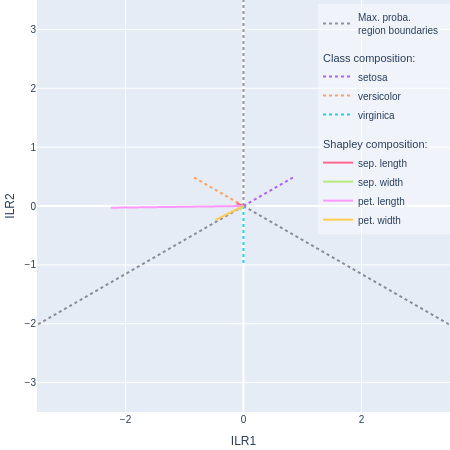
\includegraphics[width=\linewidth]{figures/3classes/ilrplot.png}
  \caption{Shapley compositions in the ILR space for an Iris instance}
  \label{fig:3classes}
\end{figure}

\subsubsection{Four classes}

...
\subsubsection{More classes}
\label{sec:more}
...

\subsection{Angles, norms and projections}

Some may find the fine analysis of the features contributions in cases with more than four classes, like discussed in Section \ref{sec:more}, tricky. Indeed, this require a careful choose of the sequential binary partition (i.e. the basis) and of the subspace to visualize. However, the Shapley explaination can be summarized by sets of angles, norms and projections.

Indeed the norm of a Shapley composition gives the strength of the contribution the feature in the prediction.

Orthogonality can also be investigated ...
...

\subsection{Histograms}

...
\subsection{About our implementation}

In this work, the estimation algorithm we used to compute the Shapley compositions is an adaptation of Algorithm 2 in \cite{vstrumbelj2014explaining}. Since the resulting Shapley compositions are approximations, the efficiency property does not necessarily hold without an adjustement. Each Shapley compositions are therefore corrected following a similar method as in the sampling approximation in the SHAP toolkit \cite{NIPS2017_7062}\footnote{\url{https://github.com/shap/shap/blob/master/shap/explainers/_sampling.py}}. See Appendix \ref{app:algo} and \ref{app:correct} for more details.


\message{ !name(main.tex) !offset(360) }

\end{document}


% This document was modified from the file originally made available by
% Pat Langley and Andrea Danyluk for ICML-2K. This version was created
% by Iain Murray in 2018, and modified by Alexandre Bouchard in
% 2019 and 2021 and by Csaba Szepesvari, Gang Niu and Sivan Sabato in 2022.
% Modified again in 2023 and 2024 by Sivan Sabato and Jonathan Scarlett.
% Previous contributors include Dan Roy, Lise Getoor and Tobias
% Scheffer, which was slightly modified from the 2010 version by
% Thorsten Joachims & Johannes Fuernkranz, slightly modified from the
% 2009 version by Kiri Wagstaff and Sam Roweis's 2008 version, which is
% slightly modified from Prasad Tadepalli's 2007 version which is a
% lightly changed version of the previous year's version by Andrew
% Moore, which was in turn edited from those of Kristian Kersting and
% Codrina Lauth. Alex Smola contributed to the algorithmic style files.

%%% Local Variables:
%%% mode: latex
%%% TeX-master: t
%%% End:
